% Copyright (c) 2022 by Lars Spreng
% This work is licensed under the Creative Commons Attribution 4.0 International License. 
% To view a copy of this license, visit http://creativecommons.org/licenses/by/4.0/ or send a letter to Creative Commons, PO Box 1866, Mountain View, CA 94042, USA.

%~~~~~~~~~~~~~~~~~~~~~~~~~~~~~~~~~~~~~~~~~~~~~~~~~~~~~~~~~~~~~~~~~~~~~~~~~~~~~~
% You can add your packages and commands to the loadslides.tex file. 
% The files in the folder "styles" can be modified to change the layout and design of your slides.
% I have included examples on how to use the template below. 
% Some of it these examples are taken from the Metropolis template.
%~~~~~~~~~~~~~~~~~~~~~~~~~~~~~~~~~~~~~~~~~~~~~~~~~~~~~~~~~~~~~~~~~~~~~~~~~~~~~~

\documentclass[
11pt,notheorems,hyperref={pdfauthor=whatever}
]{beamer}


% Copyright (c) 2022 by Lars Spreng
% This work is licensed under the Creative Commons Attribution 4.0 International License. 
% To view a copy of this license, visit http://creativecommons.org/licenses/by/4.0/ or send a letter to Creative Commons, PO Box 1866, Mountain View, CA 94042, USA.

%~~~~~~~~~~~~~~~~~~~~~~~~~~~~~~~~~~~~~~~~~~~~~~~~~~~~~~~~~~~~~~~~~~~~~~~~~~~~~~
% Add your packages and commands to this file
%~~~~~~~~~~~~~~~~~~~~~~~~~~~~~~~~~~~~~~~~~~~~~~~~~~~~~~~~~~~~~~~~~~~~~~~~~~~~~~

%~~~~~~~~~~~~~~~~~~~~~~~~~~~~~~~~~~~~~~~~~~~~~~~~~~~~~~~~~~~~~~~~~~~~~~~~~~~~~~
\RequirePackage{palatino}
\RequirePackage[utf8]{inputenc}
\RequirePackage[T1]{fontenc}

\usefonttheme{serif}

\usepackage{styles/elegantmacros}
\usefolder{styles}
\usetheme[style=blue]{elegant}

\newcommand{\makepart}[1]{ % For convenience
\part{#1} \frame{\partpage}
}

%~~~~~~~~~~~~~~~~~~~~~~~~~~~~~~~~~~~~~~~~~~~~~~~~~~~~~~~~~~~~~~~~~~~~~~~~~~~~~~

%~~~~~~~~~~~~~~~~~~~~~~~~~~~~~~~~~~~~~~~~~~~~~~~~~~~~~~~~~~~~~~~~~~~~~~~~~~~~~~
% Figures
\RequirePackage{booktabs}
\RequirePackage{colortbl}
\RequirePackage{ragged2e}
\RequirePackage{schemabloc}
%\RequirePackage{natbib}
\RequirePackage{caption}
\RequirePackage{subcaption}
\RequirePackage{tabularx}
\RequirePackage{array}
\RequirePackage{multirow}
\usepackage[
  style=alphabetic, 
]{biblatex}
\addbibresource{references.bib}
\newcolumntype{Y}{>{\centering\arraybackslash}X}

%~~~~~~~~~~~~~~~~~~~~~~~~~~~~~~~~~~~~~~~~~~~~~~~~~~~~~~~~~~~~~~~~~~~~~~~~~~~~~~

%~~~~~~~~~~~~~~~~~~~~~~~~~~~~~~~~~~~~~~~~~~~~~~~~~~~~~~~~~~~~~~~~~~~~~~~~~~~~~~
% Figures
\RequirePackage{wrapfig}
\RequirePackage{pgfplots}
\RequirePackage{graphicx}
\RequirePackage{adjustbox}
\RequirePackage{environ}
\pgfplotsset{compat=1.18}

\makeatletter
\newsavebox{\measure@tikzpicture}
\NewEnviron{scaletikzpicturetowidth}[1]{%
  \def\tikz@width{#1}%
  \def\tikzscale{1}\begin{lrbox}{\measure@tikzpicture}%
  \BODY
  \end{lrbox}%
  \pgfmathparse{#1/\wd\measure@tikzpicture}%
  \edef\tikzscale{\pgfmathresult}%
  \BODY
}
\makeatother
%~~~~~~~~~~~~~~~~~~~~~~~~~~~~~~~~~~~~~~~~~~~~~~~~~~~~~~~~~~~~~~~~~~~~~~~~~~~~~~

%~~~~~~~~~~~~~~~~~~~~~~~~~~~~~~~~~~~~~~~~~~~~~~~~~~~~~~~~~~~~~~~~~~~~~~~~~~~~~~
% Maths 
\RequirePackage{textcomp}
\RequirePackage{amsmath} 
\RequirePackage{amsthm}
\RequirePackage{mathtools}
%\RequirePackage{bbm}
%\RequirePackage{algorithm}
%\RequirePackage[osf,sc]{mathpazo}
%\RequirePackage{pifont}
%\newcommand{\xmark}{\ding{55}}%
%\numberwithin{equation}{section}
\DeclareMathOperator*{\argmax}{arg\,max}
\DeclareMathOperator*{\argmin}{arg\,min}

\setbeamertemplate{theorems}[numbered] % to number

\theoremstyle{definition}
\newtheorem{fact}{Fact}[section]
\newtheorem{examp}{Example}[section]

\theoremstyle{plain}
\newtheorem{definition}{Definition}[section]
\newtheorem{proposition}{Proposition}
\newtheorem{theorem}{Theorem}
\newtheorem{assumption}{Assumption}

\providecommand{\H}{\mathscr{H}}      
\providecommand{\E}{\mathbb{E}}
\makeatletter
\def\munderbar#1{\underline{\sbox\tw@{$#1$}\dp\tw@\z@\box\tw@}}
\makeatother

%~~~~~~~~~~~~~~~~~~~~~~~~~~~~~~~~~~~~~~~~~~~~~~~~~~~~~~~~~~~~~~~~~~~~~~~~~~~~~~
 % Loads packages and some defined commands

\title[
% Text entered here will appear in the bottom middle
]{Undecidability of First-Order Logic}

\subtitle{Solution to Entscheidungsproblem}

\author[
% Text entered here will appear in the bottom left corner
]{
    Arunachalaeshwaran V R,
    Alan Jojo
}

\institute{
    Indian Institute of Science}
\date{\today}

\begin{document}

% Generate title page
{
\setbeamertemplate{footline}{} 
\begin{frame}
  \titlepage
\end{frame}
}
\addtocounter{framenumber}{-1}

% You can declare different parts as a parentof sections
\begin{frame}{Part I: Introduction}
    \tableofcontents[part=1]
\end{frame}
\begin{frame}{Part II: Preliminaries}
    \tableofcontents[part=2]
\end{frame}
\begin{frame}{Part III: Halting Problem}
    \tableofcontents[part=3]
\end{frame}
\begin{frame}{Part IV: Proof of Undecidability of First-order Logic}
    \tableofcontents[part=4]
\end{frame}

\makepart{Introduction}

\section{Motivation}
\begin{frame}
\begin{itemize}
    \setlength\itemsep{2em}
    \item Can we have a machine that can check the proof of any mathematical statement?
    \item Can we have a machine that can prove or disprove any mathematical statement?
    \item Relationship to Godel's incompleteness theorem (contrast with Godel's completeness theorems. Especially different notions of completeness.).
    \item Primary reference: \cite{boolos2002computability}
\end{itemize}     
\end{frame}

\section{Capturing Computation}
\begin{frame}
\begin{itemize}
    \setlength\itemsep{1em}
    \item Turing Computability (captures the notion of algorithm/effective calculability) and relationship to formal languages
    \item Church-Turing Thesis: ''Every effectively calculable function is a computable function.`` (We shall use the expression "computable function" to mean a function calculable by a machine, and let "effectively calculable" refer to the intuitive idea without particular identification with any one of these definitions.) \cite{turing1938systems}
    \item Equivalent notions of computability: General recursive functions, Lambda calculus, Cyclic tag systems, Rule 110, most programming languages (might be helpful to think in terms of a computer program in a particular programming language) etc.
    \item Universal Turing Machines (crucially exploits the fact that description of a particular Turing machine is of finite size and hence be encoded as a natural number)
\end{itemize}     
\end{frame}

\section{Undecidability}
\begin{frame}
\begin{itemize}
    \setlength\itemsep{1em}
    \item Not all formal languages can be decided by a Turing machines. Examples are Halting problem, determining validity of a first-order logic formula (Church's theorem), post-correspondence problem, Hilbert's $10^{\text{th}}$ problem, etc.
    \item Existence of such languages can be seen by a simple counting argument.
    \item Existence of undecidable languages implies that certain functions are not computable (can be seen through reductions). Examples are busy beaver function, computing a solution to a set of Diophantine equations (output $\bot$ if no solutions exist), come up with a proof for a first-order logic formula (output $\bot$ if no proof exists) etc.
    \item Notion of recursive enumerability (relationship to Godel's incompleteness theorem. Use Lindenbaum extension to show that such subsets exist.).
\end{itemize}     
\end{frame}

\section{Proof sketch of Church's theorem}
\begin{frame}
    \begin{enumerate}
        \setlength\itemsep{1em}
        \item Consider a particular Turing machine and a unary encoding of its input.
        \item Encode the Turing machine and its input as a first-order logic formula in a manner such that the Turing machine halts iff first-order logic formula is valid (in fact we will be dealing specifically with implication formulas).
        \item For the sake of contradiction assume that there exists an algorithm to decide validity of any first-order logic formula.
        \item Use the previous algorithm to construct an algorithm for the Halting problem.
        \item As Halting problem is undecidable we have a contradiction.
        \item Hence, we conclude that no algorithm can decide the validity of any first-order logic formula.
    \end{enumerate}
\end{frame}

\makepart{Preliminaries}

\section{Formal Languages}
\begin{frame}
\begin{itemize}
    \setlength\itemsep{2em}
    \item We have an alphabet $\Sigma$ (we can assume WLOG $\Sigma = \{0, 1\}$. In fact assuming $\Sigma = \{1\}$ is fine as we doing computability theory and not complexity theory).
    \item A string is a finite sequence of symbols from $\Sigma$. The set of all strings is denoted by $\Sigma^*$ (Kleene closure).
    \item A language $L$ is a subset of $\Sigma^*$. That is $L \in 2^{\Sigma^*}$.
    \item We can formalize our problem and as a formal language and then worry about using some machine to decide it (i.e solve the membership problem for any string).
\end{itemize}
\end{frame}

\section{Turing Machine}
\begin{frame}
\begin{itemize}
    \setlength\itemsep{1em}
    \item The formalism under consideration defines a Turing Machine as a machine with finite control, single tape, we have unary representation of the input on the tape at the start (i.e if input is $n$ then first $n$ cells of the tape have a 1 (i.e marked or stroked) and the rest are 0 (i.e unmarked or blank)), the machine halts if it is in some state in the finite control and encounters some symbol in the table (what these states and symbols are specific to the Turing machine. The states of the finite control can be partitioned into accepting and rejecting states won't be relevant for the proof.).
    \item More formally a Turing Machine is a set of finite states $Q$, initial state $q_0$, a set of accepting states $F$ (such that $F \subseteq Q$) and a partial function $\delta : Q \times \{0, 1\} \to Q \times \{0, 1\} \times \{L, R\}$ (halt if this function is not defined at that point).
    \item Each cell position denoted by a natural number. We have a discrete timeline and we have exactly one application of the transition function in one time step.
\end{itemize}
\end{frame}

\subsection{Decider vs Enumerator (undecidable vs unrecognizable)}
\begin{frame}
\begin{itemize}
    \setlength\itemsep{1em}
    \item A particular Turing machine can decide or recognize a formal language.
    \item To decide means to solve the membership problem for any string (i.e when the Turing machine is given a string as input it halts in an accepting state if the string belongs to the language, otherwise it halts in rejecting state).
    \item To recognize means to enumerate over all strings of the language. Equivalently, partially solves i.e semidecides the membership problem (i.e when the Turing machine is given a string as input it halts in an accepting state if the string belongs to the language otherwise it rejects by either halting in a rejecting state or going into an infinite loop). Observe, that any decider for a language is also a recognizer for that language (but the converse is not necessarily true).
    \item A formal language is said to be undecidable if there is no Turing that decides that language.
    \item A formal language is said to be unrecognizable if there is no Turing that decides that language.
\end{itemize}
\end{frame}

\subsection{Encoding a Turing Machine as a Finite String}
\begin{frame}
\begin{itemize}
    \setlength\itemsep{3em}
    \item Observe that description of a Turing machine only consists of $Q$, $q_0$, $F$, $\delta$; as all of them are finite we can give description of a Turing machine as a finite string.
    \item Intuitively this finite string can be seen as the "source code" of the Turing machine.
\end{itemize}
\end{frame}

\subsection{Universal Turing Machine}
\begin{frame}
\begin{itemize}
    \setlength\itemsep{3em}
    \item There exist Turing machines with the property that they take as input description of a Turing machine, input string and can simulate it on the input string. Such Turing machines are called universal Turing machines.
    \item These universal Turing machines can be intuitively seen as interpreters (an explicit construction of a Turing machine is not provided here).
\end{itemize}
\end{frame}

\subsection{Complement of a language}
\begin{frame}
\begin{itemize}
    \setlength\itemsep{3em}
    \item Complement of a formal language $L$ is $\Sigma^* \setminus L$. Complement of language $L$ will be denoted by $\overline{L}$.
    \item If both $L$ and $\overline{L}$ are recognizable then $L$ is decidable.
    \item If $L$ is undecidable then $L$ or $\overline{L}$ is unrecognizable (contrapositive of the previous point).
\end{itemize}
\end{frame}

\section{Robinson Arithmetic}
\begin{frame}
\begin{itemize}
    \setlength\itemsep{2em}
    \item Essentially Peano arithmetic without the axiom schema of induction.
    \item Every computable function can be represented in Robinson arithmetic. \cite{odifreddi1992classical} (Using this along side diagonalization will help us prove Godel's incompleteness theorem)
    \item Robinson arithmetic (denoted by $\textbf{Q}$ is essentially undecidable i.e every consistent extension is undecidable. Theory of fields is undecidable but not essentially undecidable.)
    \item It is a handy tool for proving incompleteness theorems and other limitative results. \footnote{\url{http://www.columbia.edu/~jc4345/Notes\%20on\%20Incompleteness\%20Theorems.pdf}}
\end{itemize}
\end{frame}

\subsection{Signature}
\begin{frame}
\begin{itemize}
    \setlength\itemsep{2em}
    \item $S^{(1)}$ is intuitively the successor function
    \item $+^{(2)}$ is intuitively the addition function
    \item $\cdot^{(2)}$ is intuitively the multiplication function
    \item $0$ is intuitively the constant zero i.e additive identity
    \item $1$ is intuitively the constant one i.e multiplicative identity
\end{itemize}
\end{frame}

\subsection{Axioms}
\begin{frame}
    \begin{enumerate}
        \setlength\itemsep{2em}
        \item $Sx \not= 0$ (zero is not the successor of any number)
        \item $(Sx = Sy) \implies x = y$ (if successors of two numbers are equal then the two numbers are equal)
        \item $y = 0 \vee \exists_x (Sx = y)$ (Every number is either 0 or has a predecessor i.e is a successor of some number)
        \item $x + 0 = x$ (Recursive definition of addition base case. Also, can be interpreted as $0$ is additive right identity)
        \item $x + Sy = S(x+y)$ (Recursive definition of addition main case)
        \item $x \cdot 0 = 0$ (Recursive definition of multiplication base case. Also, can be interpreted as $0$ is multiplicative right identity)
        \item $x \cdot Sy = x \cdot y + x$ (Recursive definition of multiplication main case)
    \end{enumerate}
\end{frame}

\section{Godel's Incompleteness Theorem}
\begin{frame}
\begin{itemize}
    \setlength\itemsep{1em}
    \item Does not contradict the Godel's completeness theorem. As different notions of completeness is used in the two theorems.
    \item \textbf{Godel's first incompleteness theorem: } Any consistent formal system $F$ (formal system $F$ means the theorems of $F$ are recursively enumerable) within which a certain amount of elementary arithmetic (Robinson arithmetic) can be carried out is incomplete; i.e., there are statements of the language of $F$ which can neither be proved nor disproved in $F$. \cite{raatikainen2013godel}
    \item \textbf{Godel's second incompleteness theorem: } For any consistent formal system $F$ within which a certain amount of elementary arithmetic (Robinson arithmetic) can be carried out, the consistency of F cannot be proved in $F$ itself. \cite{raatikainen2013godel}
    \item We need to consider the possibility of undecidability only because incompleteness theorems exist (any incompleteness theorem will do for this purpose and not just Godel's incompleteness theorems).
\end{itemize}
\end{frame}

\makepart{Halting Problem}

\section{Statement of Halting Problem}
\begin{frame}
\begin{itemize}
    \setlength\itemsep{1em}
    \item Give a Turing machine to decide the following language $K = \{(i, x) | \text{ program } i \text{ halts when run on input } x\}$.
    \item Essentially we must determine whether a particular Turing machine halts on a particular input or not.
    \item In set above $i$ is the finite string representation of the particular Turing machine and $x$ is the finite string representation of the particular input.
    \item We need to determine whether the Turing machine represented by $i$ halts on input $x$ or not.
    \item \textbf{Note: } If $i$ is not a valid representation of a Turing machine then map it some arbitrary Turing machine say the Turing machine that accepts on all inputs.
\end{itemize}
\end{frame}

\section{Proof of Undecidability of Halting Problem}
\begin{frame}
\begin{enumerate}
    \item For the sake of contradiction lets assume that there is a computable function $$h(i, x) = \begin{cases}
  1 & \text{if } \text{  program }i\text{ halts on input }x, \\
  0 & \text{otherwise.}
\end{cases}$$. Observe, that existence of $h$ is equivalent to saying there exists Turing machine that can decide the language $K$.
    \item Now, for any computable function $f$ taking two arguments (later we show that $h$ can't be such a function to obtain a contradiction. Also, arity is not that important as we can change arity effectively arbitrarily.) consider the function $$g(i) = \begin{cases}
  0  & \text{if } f(i,i) = 0,\\
  \text{undefined} & \text{otherwise.}
\end{cases}$$ and the program $e$: Refer Figure \ref{fig:program_e} \footnote{Proof and Image Credits: \url{https://en.wikipedia.org/wiki/Halting\_problem}}
    \item Overloaded $e$ to be both the name of the function and the representation of the function.
\end{enumerate}
\end{frame}

\subsection{Proof continuation}
\begin{frame}

\begin{figure}
    \centering
    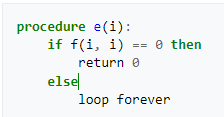
\includegraphics{images/program.png}
    \caption{Program $e$}
    \label{fig:program_e}
\end{figure}

\begin{enumerate}
    \setcounter{enumi}{3}
    \item Now, there are only two cases to consider (by the definition of $g$):-
    \begin{enumerate}
        \item $f(e, e) = 0$. Therefore, $g(e) = 0$. Machine represented by $e$ halts on input $e$ so $h(e, e) = 1$.
        \item $f(e, e) \not= 0$. Therefore, $g(e)$ is undefined. Machine represented by $e$ does not halt on input $e$ therefore $h(e, e) = 0$.
    \end{enumerate}
    \item In the both cases considered above $f(e, e) \not= h(e, e)$. Therefore, $h$ does not output the same value as any $f$ ($f$ can be any computable function taking two arguments).
    \item Therefore $h$ is not computable. A contradiction.
    \item Therefore, the Halting problem is undecidable.
\end{enumerate}
\end{frame}

\makepart{Proof of Undecidability of First-Order Logic}

\section{Introduction}
\begin{frame}
\begin{itemize}
    \setlength\itemsep{2em}
    \item Turing's Thesis - The halting problem is not solvable by any Turing machine.
    \item Given the machine table of a Turing machine, and any $n$, we can effectively write down a finite set of sentences $\Gamma$ and a sentence $D$ such that $\Gamma$ implies $D$ if and only if the machine does eventually halt when started with input $n$.
    \item It follows that if the decision problem for logical implication could be solved, then the halting problem for Turing machines could be solved.
    \item So assuming Turing's thesis, the decision problem is unsolvable.
\end{itemize}
\end{frame}

\section{Intuitive Explanation of the Logic's Signature}
\begin{frame}
\begin{itemize}
    \item The domain of $\mathcal{M}$ will in all cases be the integers, positive and zero and negative.
    \item The nonnegative integers will be used to number the times when the machine is operating. The machine starts at time 0.
    \item The integers will also be used to number the squares on the tape. The machine starts at square 0.
    \begin{figure}
        \centering
        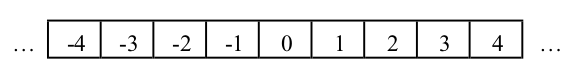
\includegraphics[scale=0.5]{images/01_tape.png}
        \caption{Numbering the squares of a Turing tape}
        \label{fig:turing_tape}
    \end{figure}
    \item Constant $\pmb{0}$ - denotes zero in standard interpretation
    \item Predicate $\pmb{S}$ will denote the successor relation. We denote $\pmb{S}(u,v)$ by $\pmb{S}uv$.
    \item Predicate $\pmb{<}$ will denote the usual order relation. We denote $\pmb{<}(u,v)$ by $u \pmb{<}v$.
    \item For each of the $k$ (nonhalted) states of the machine define a one-place predicate $\pmb{Q}_i\quad 1<i<k$.\\
    $\pmb{Q}_i$ will denote the set of $t\ge 0$ such that at the time $t$ the machine is in the state $i$.
    \item Predicate $\pmb{L}$ will denote the set of pairs of integers $t\ge 0$ and $x$ such that at the time $t$, the machine is at the square $x$.
    \item Predicates $\pmb{M}_e$ ($e=0$ or $1$) will denote the set of pairs of integers $t\ge 0$ and $x$ such that at the time $t$, square $x$ contains symbol $e$.
\end{itemize}
\end{frame}

\section{Intuitive Explanation of the Formula}
\begin{frame}
$\Gamma$ will consist of 3 groups of sentences:
\begin{enumerate}
    \setlength\itemsep{0.5em}
    \item[(a)] Background information about $\pmb{S}$ and $\pmb{<}$ that would be the same for any machine and any input
    \item[(b)] A single sentence specific to the input $n$ we are considering
    \item[(c)] One sentence for each ‘normal’ instruction (except for halt instruction) of the specific machine we are considering
\end{enumerate}
\vspace{3em}
$D$ will be the disjunction of all halting instruction sentences.
\end{frame}

\subsection{Sentences in $\Gamma(a)$ Eq. (1)-(3)}
\begin{frame}
Background information:
\vspace{3em}
\begin{enumerate}
    \setlength\itemsep{1em}
    \item[(1)] $\forall u\forall v\forall w(((\pmb{S}uv \wedge \pmb{S}uw) \to v = w) \wedge ((\pmb{S}vu \wedge \pmb{S}wu) \to v = w))$
    \item[(2)] $\forall u\forall v(\pmb{S}uv \to u \pmb{<} v) \wedge \forall u\forall v\forall w((u \pmb{<} v \wedge v \pmb{<} w \to u \pmb{<} w)$
    \item[(3)] $\forall u\forall v(u\pmb{<}v \to u \pmb{\neq} v)$
\end{enumerate}
\end{frame}

\subsection{Sentences in $\Gamma(a)$ Eq. (4)-(8)}
\begin{frame}
\begin{itemize}
    \setlength\itemsep{2em}
    \item Abbreviations for the $m$th-successor relation
    \vspace{0.5em}
    \begin{itemize}
        \setlength\itemsep{0.8em}
        \item $\pmb{S}_0 uv$ for $u=v$
        \item $\pmb{S}_1 uv$ for $\pmb{S} uv$
        \item $\pmb{S}_2 uv$ for $\exists y(\pmb{S}uy \wedge \pmb{S}yv)$
        \item $\pmb{S}_3 uv$ for $\exists y_1\exists y_2(\pmb{S}uy_1 \wedge \pmb{S}y_1 y_2) \wedge \pmb{S}y_2 v$
    \end{itemize}
    \item In the standard interpretation, the following are true:
    \vspace{0.5em}
    \begin{enumerate}
        \setlength\itemsep{0.8em}
        \item[(4)] $\forall u\forall v\forall w(((\pmb{S}_m uv \wedge \pmb{S}_m uw) \to v = w) \wedge ((\pmb{S}_m vu \wedge \pmb{S}_m wu) \to v = w))$
        \item[(5)] $\forall u\forall v(\pmb{S}_m uv \to u \pmb{<} v)$ if $m\neq 0$
        \item[(6)] $\forall u\forall v(\pmb{S}_m uv \to u \pmb{\neq} v)$ if $m\neq 0$
        \item[(7)] $\forall u\forall v\forall w((\pmb{S}_m wu \wedge \pmb{S} uv) \to \pmb{S}_k wv) \qquad \text{if} \quad k=m+1$
        \item[(8)] $\forall u\forall v\forall w((\pmb{S}_k wv \wedge \pmb{S} uv) \to \pmb{S}_m wu) \qquad \text{if} \quad m=k-1$
    \end{enumerate}
\end{itemize}
\end{frame}

\subsection{Sentences in $\Gamma(a)$ Eq. (9)-(11)}
\begin{frame}
We will write
\vspace{0.5em}
\begin{itemize}
    \setlength\itemsep{1em}
    \item $y=\pmb{1}$ for $\pmb{S}_1(\pmb{0},y)$ and $y=\pmb{-1}$ for $\pmb{S}_1(y,\pmb{0})$
    \item $\pmb{Q}_i\pmb{2}$ for $\exists y(y=\pmb{2}\wedge Q_i y)$
    \item $\pmb{S2}u$ for $\exists y(y=\pmb{2}\wedge \pmb{S}yu)$
\end{itemize}
\vspace{3em}
Assume that $p,q,m,k$ are the numerals for the numbers $p,q,m,k$. Then
\vspace{0.5em}
\begin{enumerate}
    \setlength\itemsep{1em}
    \item[(9)] $\pmb{p}\neq\pmb{q}\qquad\text{if}\quad p\neq  q$
    \item[(10)] $\forall v(\pmb{Sm}v \to v = \pmb{k})\qquad\text{where}\quad k=m+1$
    \item[(11)] $\forall u(\pmb{S}u\pmb{k} \to u = \pmb{m})\qquad\text{where}\quad m=k-1$
\end{enumerate}
\end{frame}

\subsection{Sentences in $\Gamma(b)$}
\begin{frame}
A single sentence specific to the input $n$
\vspace{3em}
\begin{enumerate}
    \item[(12)] $\pmb{Q_0 0}\wedge \pmb{L00} \wedge \pmb{M_100} \wedge \pmb{M_101} \wedge \cdots  \wedge \pmb{M_1\ 0\ n-1} \wedge \forall x((x\neq\pmb{0}\wedge x\neq\pmb{1}\wedge \cdots\wedge x\neq\pmb{n-1})\to \pmb{M_0 0}x)$
\end{enumerate}
\vspace{3em}
At time $0$ the machine is in state 1, at square 0, with squares $0$ through $n-1$ marked to represent the input $n$, and all other squares blank.
\end{frame}

\subsection{Sentences in $\Gamma(c)$}
\begin{frame}
There will be one sentence for each nonhalting instruction. For each instruction of the following form, where $j$ is not the halted state
\vspace{1em}
\begin{enumerate}
    \item[(*)] If you are in state $i$ and are scanning symbol $e$, then ------ and go into state $j$.
\end{enumerate}
\vspace{1em}
there will be a sentence. This sentence will have the following form:
\vspace{1em}
\begin{enumerate}
    \item[(13)] $\forall t\forall x((\pmb{Q}_i t \wedge \pmb{L}tx \wedge \pmb{M_e}tx)\to$\\$\exists u(\pmb{S}tu\wedge \text{------} \wedge \pmb{Q_j}u \wedge \forall y((y\neq x \wedge \pmb{M_1}ty)\to\pmb{M_1}uy)\wedge\forall y((y\neq x\wedge \pmb{M_0}ty)\to\pmb{M_0}uy)))$
\end{enumerate}
\vspace{1em}
The marking of squares other than $x$ remains unchanged from one time $t$ to the next time $u$.\\
If the space ‘——----’ in (*) is filled by
\begin{itemize}
    \item Print the symbol $d$, then ‘——----’ in (13) is filled by $\pmb{L}ux \wedge \pmb{M}_d ux$
    \item Move one square to right, then ‘——----’ in (13) is filled by $\exists y(\pmb{S}_1 xy \wedge \pmb{L}uy \wedge (\pmb{M}ux\leftrightarrow\pmb{M}tx))$
    \item Move one square to left, then ‘——----’ in (13) is filled by $\exists y(\pmb{S}_{-1} xy \wedge \pmb{L}uy \wedge (\pmb{M}ux\leftrightarrow\pmb{M}tx))$
\end{itemize}
\end{frame}

\subsection{Section D}
\begin{frame}
    
\end{frame}

\section{Completing the Proof}
\begin{frame}
\end{frame}

\begin{frame}[allowframebreaks]{References}
    \printbibliography
\end{frame}
\end{document}